
\chapter{Implementación}
\label{chap:implementación}

La idea no es implementar un sistema production ready, pero si verificar que as comunicaciones funcionan correctamente. En este capitulo describiremos la implementación de las capas de conocimiento y nivel del bucle. Dejaremos para más adelante, el capitulo \ref{chap:caso_estudio} la descripción de la implementación del nivel de solución y sistema manejado. En este capitulo ofrecemos una vista más concreta de la implementación, y las tecnologías empleadas. EN el otro describiremos cómo encaja todo a nivel general y veremos cómo opera.

Una vez descrito el diseño del sistema, llegamos a la etapa de implementación. Aunque no era uno de los objetivos del trabajo, optamos por implementar un sistema básico que siga el diseño. De esta forma pudimos verificar la distribución de los componentes, verificar la viabilidad de los conectores y refinar los protocolos de comunicación. La implementación fue incremental, y el diseño fue evolucionando según detectábamos nuevas necesidades o problemas que no resolvía nuestra arquitectura. Así pudimos validar qué funcionaba y que no.

La implementación se llevo a cabo en 4 hitos distintos, cada uno correspondiente a una etapa distinta del bucle:
\begin{itemize}
  \item \textbf{Hito 1 - Servicio de monitorización y conocimiento}:
  \item \textbf{Hito 2 - Servicio de análisis y reglas}
  \item \textbf{Hito 3 - Planificador}
  \item \textbf{Hito 4 - Ejecutor y efectores}
\end{itemize}

En esta primera etapa acordamos implementar el proceso de registro de las medidas de una sonda, hasta que se graba en el conocimiento. Esto implicó implementar las sondas y monitores del caso de estudio (capitulo \ref{chap:caso_estudio}), el componente de monitorización del bucle MAPE-K y la base de conocimiento. Se comenzó también con el prototipado de los que se convertirían en los conectores para comunicaciones descendentes: los conectores de APIs REST.

El objetivo era implementar desde que la sonda reporta una medida hasta que se almacena esta nueva medida en el conocimiento. Para ello tuvimos que implementar la comunicación entre la sonda y el monitor de la solución. Después del monitor de la solución al componente de monitorización del bucle. Y de este último al conocimiento. La implementación de todos ellos fue muy parecida.

Respecto a los servicios, se optó por implementar el sistema con servicios en ASP.NET\footnote{Página oficial: \url{https://docs.microsoft.com/en-us/aspnet/core/introduction-to-aspnet-core}}. Se trata de un \emph{framework} para implementar servidores web de la plataforma .NET de Microsoft. Como comentamos en la sección \ref{chap:OpenAPI}, estos servicios expondrán \foreign{english}{endpoints} HTTP. En el listing \ref{ls:csharp-get} ya mostramos un ejemplo de la implementación de estos \foreign{english}{endpoints}.

A partir de estos endpoints, gracias al uso de la librería \emph{Swashbuckle.AspNetCore}\footnote{Página oficial: \url{https://github.com/domaindrivendev/Swashbuckle.AspNetCore}}, pudimos generar la especificación de nuestros servicios en el estándar OpenAPI. Esto nos aporta dos cosas: una interfaz de usuario para interactuar con la API y la posibilidad de generar el API client.

Hablemos primero sobre la interfaz de usuario. La librería añade a nuestro servicio el \emph{endpoint} \texttt{/swagger}. Accediendo a esta ruta, el servicio nos presentará una interfaz con un listado de todas las operaciones que ofrece la API Rest. De cada petición nos muestra su documentación (la que añadimos en el código), sus parámetros y nos permite incluso ejecutarla allí mismo. De esta forma, nuestros usuarios pueden hacer pruebas de las peticiones antes de implementar su propio cliente. O para situaciones de emergencia cuando necesitemos ejecutar una petición por algún motivo (depuración?)

\begin{figure}[htb]
  \centering
  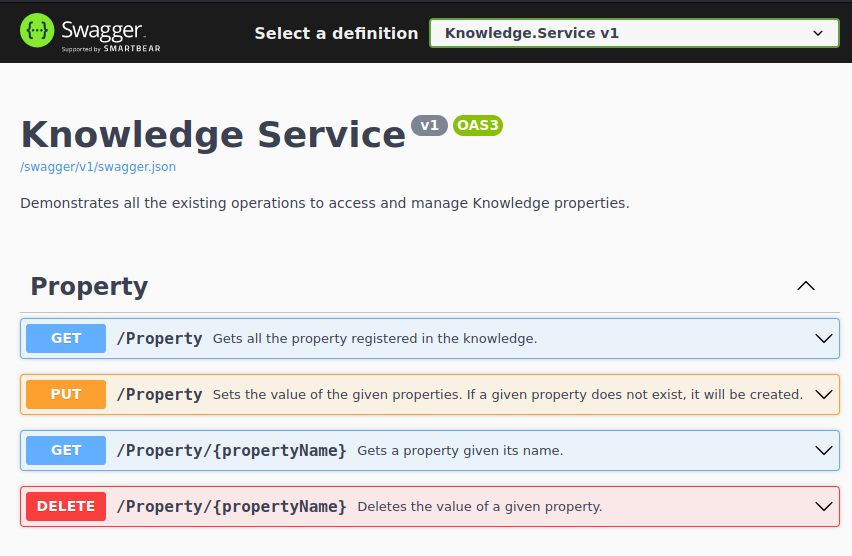
\includegraphics[scale=1.5]{cap_implementacion/images/swagger-knowledge-ui}
  \caption{Interfaz de usuario ofrecida por Swagger para el servicio de conocimiento. Se genera a partir de las especificación OpenAPI.}
  \label{fig:swagger-knowledge-ui}
\end{figure}

Por otro lado, también nos permite generar el API Client. Como comentamos en la sección de OpenAPI, tenemos gran variedad de generadores de código a nuestra disposición. Nosotros optamos por los ofrecidos por la librería \texttt{OpenApi.Generators}\footnote{Página del proyecto: \url{https://github.com/OpenAPITools/openapi-generator}}. En concreto, el generador de código de \verb|C#|. Usándolo, pudimos generar una librería que permite contactar con nuestro servicio, sin necesidad de implementar mucho código. Por ejemplo, el componente de monitorización del bucle contacta a través del bucle MAPE-K a través del API Client generado.

El módulo del conocimiento es un servicio muy sencillo. Para esta implementación de referencia optamos por implementarlo con un diccionario en memoria, que asigna los pares clave-valor. Esto nos permite direccionarlas y acceder desde fuera a estos recursos. Ofrece operaciones de lectura y escritura sobre estas propiedades y configuraciones de servicio.

Por encima de este, tenemos el módulo de monitorización. Actúa como intermediario entre los monitores de la solución y el conocimiento. También cuenta con una implementación muy sencilla. Ofrece operaciones de lectura de propiedades del conocimiento y para los monitores de la solución reporten medidas. De esta forma, los monitores de solución podrán obtener los valores de otras propiedades y valor si deben permitir o no la escritura de esa medida.

\textcolor{red}{¿Añadir ejemplo? ¿Desribir los componentes implementados? ¿Debería describirse el caso de uso con la implementación del bucle MAPE-K?}

\subsubsection{Hito 2: Servicio de análisis y reglas.}

En el segundo hito, acordamos implementar la evaluación de reglas de adaptación. Esto requería de implementar el módulo de análisis del bucle MAPE-K y los módulos de reglas de la solución. Además, fue cuando empezamos a plantearnos el diseño de las notificaciones, las comunicaciones ascendentes. Así evitábamos que se acoplaran los componentes entre sí.

Primero describiremos este mecanismo de notificación. Una vez se confirma la escritura de una propiedad o configuración en el conocimiento, este publica un \textbf{evento de integración} (fanout) que llega a todos los suscriptores de estén en la capa superior. Optamos por implementar estas operaciones con \texttt{RabbitMQ}\footnote{Página oficial: \url{https://www.rabbitmq.com/}}. Se trata de un broker de mensajería ''sencillo'' ampliamente utilizado. Nos permite implementar los dos patrones que necesitamos: las notificaciones y las peticiones asíncronas.

Además, para implementar nuestro conector de forma agnóstica a la tecnología usada, utilizamos una librería llamada \texttt{Rebus}\footnote{Página oficial: \url{https://github.com/rebus-org/Rebus}}. Esta nos permite implementar comunicaciones con un bus, abstrayéndonos de la tecnología concreta utilizada para la comunicación.

\textcolor{red}{Dibujo que represente RabbitMQ y rebus.}

En cuanto a la implementación del módulo de análisis, este realmente no tiene mucha lógica. Participa como intermediario entre el conocimiento y los módulos de reglas. Esto nos permitía abstraer a las reglas del acceso al conocimiento, y en un futuro, añadir mecanismos de autenticación y autorización para protegerlos.

Por otro lado, también traducen las notificaciones del módulo de conocimiento
